\section{Extended Kalman Filter}

Consider a state-space model with nonlinear dynamics:
\[\mathcal{S}:\begin{cases}
    \mathbf{x}(t+1)=f(\mathbf{x}(t),\mathbf{u}(t))+\mathbf{v}_1(t) \\
    \mathbf{y}(t)=h(\mathbf{x}(t))+\mathbf{v}_2(t)
\end{cases}\]
Here, $f(\cdot)$ and $h(\cdot)$ are nonlinear functions of class $C^1$ or higher.

The Extended Kalman Filter is a variant of the Kalman Filter designed to handle nonlinear dynamics and measurements. 
It approximates the nonlinear system by linearizing it at each time step around the current estimate of the state.
To illustrate the idea, let's consider the following block diagram of the Extended Kalman Filter:
\begin{figure}[H]
    \centering
    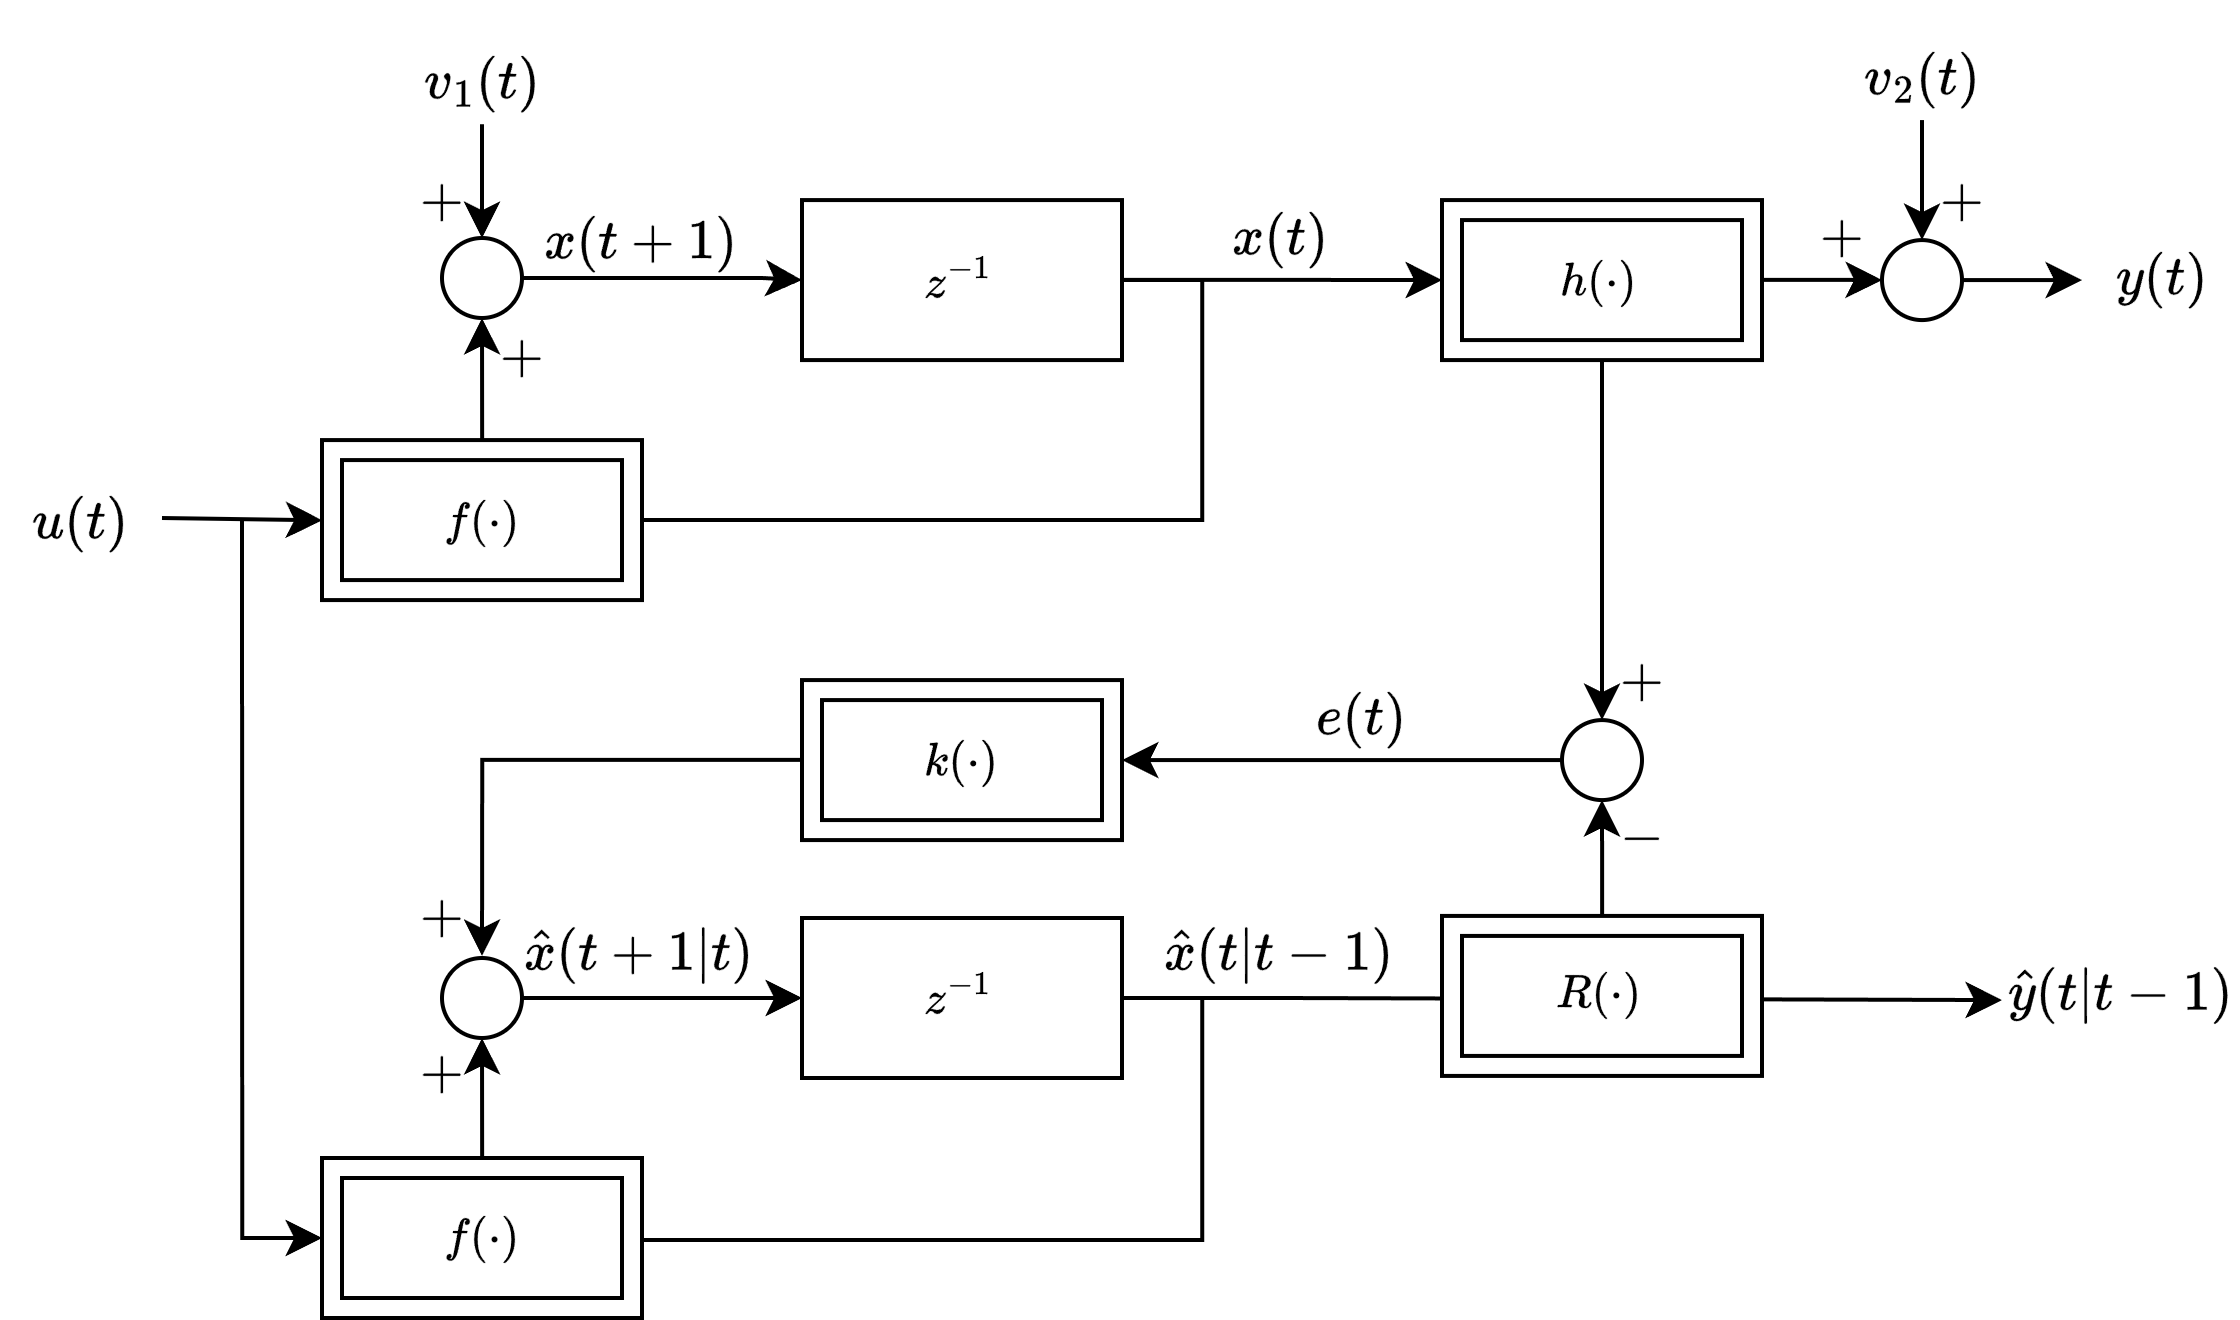
\includegraphics[width=0.75\linewidth]{images/ekf.png}
    \caption{Extended Kalman Filter block scheme}
\end{figure}
To establish the feedback correction gain, we have two distinct options:
\begin{enumerate}
    \item The gain is structured as a nonlinear function, denoted as $\mathbf{K}(\cdot)$, yielding an output of $\mathbf{K}(\mathbf{e}(t))$. 
    \item Alternatively, the gain takes the form of a linear time-variant block akin to the Kalman Filter, producing an output of $\mathbf{K}(t)\mathbf{e}(t)$. 
\end{enumerate}
The Extended Kalman Filter embraces the latter approach, albeit less intuitive, it proves more efficacious by leveraging established theory from traditional Kalman Filters.

To easily compute the gain $\mathbf{K}(t)$ using the Kalman Filter formula, we utilize the usual equations.
To implement this formula, we require a method for computing $\mathbf{F}(t)$ and $\mathbf{H}(t)$ at each sampling instant:
\[\mathbf{F}(t)=\dfrac{\partial f(\mathbf{x}(t),\mathbf{u}(t))}{\partial \mathbf{x}(t)} \qquad \mathbf{H}(t)=\dfrac{\partial h(\mathbf{x}(t))}{\partial \mathbf{x}(t)}\]
These derivatives are assessed at $\mathbf{x}(t)=\hat{\mathbf{x}}(t\mid t-1)$. 
Hence, $\mathbf{F}(t)$ and $\mathbf{H}(t)$ become time-varying matrices acquired through the local linearization of the nonlinear system around the predicted state vector from the preceding step.

In practice, the Extended Kalman Filter aims to convert a nonlinear, time-invariant system into a linear, time-varying system. 
Subsequently, it employs the Kalman Filter methodology on this transformed linear system.

The general procedure for the Extended Kalman Filter at the current time $t$ is outlined as follows:
\begin{enumerate}
    \item Utilize the most recent state prediction, denoted as $\hat{\mathbf{x}}(t\mid t-1)$. 
    \item Employ $\hat{\mathbf{x}}(t\mid t-1)$ to compute $\mathbf{F}(t)$ and $\mathbf{H}(t)$. 
    \item Calculate $\mathbf{K}(t)$  and update the Differential Riccati Equation, thereby determining $\mathbf{P}(t+1)$. 
    \item Compute $\hat{\mathbf{x}}(t+1\mid t)$ for the subsequent iteration.
\end{enumerate}
This iterative procedure must be repeated for each sampling instant. 

\paragraph*{Remarks}
The Extended Kalman Filter stands out for its efficacy in handling nonlinear systems. 
However, due to its inherent nature as a nonlinear, time-variant system, it lacks a steady-state solution. 
Consequently, several implications arise:
\begin{itemize}
    \item Achieving asymptotic stability is challenging or infeasible, necessitating extensive empirical validation.
    \item Computational burden: with each sampling instance, recalculations of $\mathbf{F}(t)$, $\mathbf{H}(t)$, $\mathbf{P}(t)$, and $\mathbf{K}(t)$ are required.
\end{itemize}
While the Extended Kalman Filter finds widespread application, it encounters limitations in scenarios involving safety critical systems and applications, and mission critical systems and applications. 
The exploration of meta-parameters within the Kalman Filter structure represents a new avenue in Machine Learning.